\begin{filecontents*}{mybib.bib}
@book{Sutton2018,
  added-at = {2019-07-13T10:11:53.000+0200},
  author = {Sutton, Richard S. and Barto, Andrew G.},
  biburl = {https://www.bibsonomy.org/bibtex/2f46601cf8b13d39d1378af0d79438b12/lanteunis},
  edition = {Second},
  interhash = {ac6b144aaec1819919a2fba9f705c852},
  intrahash = {f46601cf8b13d39d1378af0d79438b12},
  keywords = {},
  publisher = {The MIT Press},
  timestamp = {2019-07-13T10:11:53.000+0200},
  title = {Reinforcement Learning: An Introduction},
  url = {http://incompleteideas.net/book/the-book-2nd.html},
  year = {2018 }
}
\end{filecontents*}

\documentclass[10pt,a4paper]{article}
\usepackage[utf8]{inputenc}
\usepackage[top=1.25in, bottom=1.25in, left=.75in, right=.75in]{geometry}
\usepackage{amsmath}
\usepackage{algorithmicx}
\usepackage{algpseudocode}
\usepackage{algorithm2e}
\usepackage{amsfonts}
\usepackage{mathtools}
\usepackage{amssymb}
\usepackage{xcolor}
\usepackage{natbib}
\usepackage{bibentry}
\usepackage{fancyhdr}
\usepackage{dsfont}
\renewcommand{\familydefault}{\sfdefault}
\pagestyle{fancy}
\lhead{Exercise sheet \#2}
\nobibliography*
\DeclareMathOperator*{\argmax}{arg\,max}
\author{Johannes Ender}
\begin{document}
\clearpage
\setcounter{section}{2}
\section{Dynamic Programming}
\subsection*{22. Exercise 4.1 In Example 4.1, if $\pi$ is the equiprobable random policy, what is $q_\pi$(11, down)?}
As the terminal state's action value is 0, $q_\pi$(11, down) can be calculated as:
\begin{align*}
q_\pi(11, down) &= p(s', r \mid s, a)[r] \\
&= 1 \cdot [-1] = -1
\end{align*}

\subsection*{23. Exercise 4.2 In Example 4.1, suppose a new state 15 is added to the gridworld just below state 13, and its actions, left, up, right, and down, take the agent to states 12, 13, 14, and 15, respectively. Assume that the transitions from the original states are unchanged. What, then, is $v_\pi(15)$ for the equiprobable random policy? Now suppose the dynamics of state 13 are also changed, such that action down from state 13 takes the agent to the new state 15. What is $v_\pi(15)$ for the equiprobable random policy in this case?}
Using the general formula
\begin{align*}
v_\pi(s) = \sum_a \pi(a \mid s) \sum_{s', r} p(s', r \mid s, a)[r + \gamma v_\pi(s')]
\end{align*}
$v_\pi(15)$ can be calculated as
\begin{align*}
v_\pi(15) &=\frac{1}{4} p(12, -1 \mid 15, left)[-1 + \gamma v_\pi(12)] + \\
&\frac{1}{4} p(13, -1 \mid 15, up)[-1 + \gamma v_\pi(13)] + \\
&\frac{1}{4} p(14, -1 \mid 15, right)[-1 + \gamma v_\pi(14)] + \\
&\frac{1}{4} p(15, -1 \mid 15, down)[-1 + \gamma v_\pi(15)] \\
&= -1 + \frac{1}{4} v_\pi(12) + \frac{1}{4} v_\pi(13) + \frac{1}{4}v_\pi(14) + \frac{1}{4}v_\pi(15)
\end{align*}

\subsection*{25. Exercise 4.3 What are the equations analogous to (4.3), (4.4), and (4.5) for the action-value function $q_\pi$ and its successive approximation by a sequence of functions $q_0$ , $q_1$ , $q_2$ ,... ? (Textbook p. 74)}
\begin{align*}
q_\pi(s, a) &= \mathbb{E}_\pi[G_t \mid S_t = s, A_t = a] = \mathbb{E}_\pi[R_{t+1} + \gamma q_\pi(S_{t+1}, A_{t+1}) \mid S_t = s A_t = a] \\
&= \sum_{s', r} p(s', r \mid s, a)[r + \gamma q_\pi(s', a)] \\ \\
q_{k+1}(s, a) &= \sum_{s', r} p(s', r \mid s, a)[r + \gamma q_k(s', a')]
\end{align*}

\newpage
\subsection*{26. 6. Exercise 4.5 How would policy iteration be defined for action values? Give a complete algorithm for computing $q_\ast$, analogous to that on page 80 for computing $v_\ast$. Please pay special attention to this exercise, because the ideas involved will be used throughout the rest of the book.}
\begin{align*}
\pi_0 \xrightarrow{pe} q_{\pi_0} \xrightarrow{pi} \pi_1 \xrightarrow{pe} q_{\pi_1} \cdots \xrightarrow{pi} \pi_\ast \xrightarrow{pe} q_\ast
\end{align*}


\RestyleAlgo{boxruled}
\begin{algorithm}[ht]
\textbf{1. Initialization}\\
$\pi \leftarrow \text{arbitrary deterministic policy}$\\
$Q \leftarrow \text{arbitrary}$ \\
$\theta \leftarrow \text{small positive number}$ \\
\vspace{.5cm}
\textbf{2. Policy evaluation}\

 \While{$\Delta < \theta$}{
	\For{ each s $\epsilon\; \mathcal{S}$ and $a\; \epsilon\; \mathcal{A}(s)$}
	{
		$q \leftarrow Q(s, a)$ \\
		$q(s,a) \leftarrow \sum_{s', r} p(s', r \mid s, a)[r + \gamma q_\pi(s', a)]$\\
		$\Delta \leftarrow max(\Delta, \mid q - Q(s,a)\mid)$
	}
 }
 \vspace{1cm}
 \textbf{3. Policy improvement} \\
 $improved \leftarrow false$ \\
 \For{each $s\; \epsilon\; \mathcal{S}$}
 {
	$b \leftarrow \pi_s$ \\
	$\pi_s \leftarrow argmax_a Q(s, a)$\\
	\If{$b \neq \pi(s)$}
	{
		$improved \leftarrow true$	
	}
 }
 \If{improved}
 {
	\texttt{Goto} \textit{Policy evaluation} 
 }
 \caption{Policy iteration}
\end{algorithm}

\subsection*{27. Exercise 4.6 Suppose you are restricted to considering only policies that are $\epsilon$-soft, meaning that the probability of selecting each action in each state, s, is at least $\epsilon/|A(s)|$. Describe qualitatively the changes that would be required in each of the steps 3, 2, and 1, in that order, of the policy iteration algorithm for $v_\ast$ (Textbook p. 80).}
\textbf{Step 3:}
\\
The update of the policy would have to be changed, such that with a probability of $\epsilon / |A(s)|$ a non-greedy action is taken and the greedy action is taken with the remaining probability.\\
The check for stability of the policy, i.e. the comparison to \textit{old-action}, would have to adapted, such that for one does compare the actions with the highest probabilities.
\\
\textbf{Step 2:}
\\
In the policy evaluation, the update to the state-value function would have to be changed, s.t. it is calculated in a way similar to equation 4.5 in \cite{Sutton2018}.
\\
\textbf{Step 1:}
The initialization of the policy would have to be changed to create an $\epsilon$-soft policy.

\subsection*{28. Exercise 4.10 What is the analog of the value iteration update (4.10) for action values, $q_{k+1}(s, a)$?}
\begin{align*}
q_{k+1}(s, a) &= \mathbb{E}[r_{t+1} + \gamma max_{a'} q_k(s_{t+1}, a) \mid s_t = s, a_t = a]\\ 
&= \sum_{s', r} p(s', r \mid s, a)[r + \gamma max_{a'} q_k (s', a')]
\end{align*}
\newpage
\section{Monte Carlo Methods}
\subsection*{29. Exercise 5.3 What is the backup diagram for Monte Carlo estimation of $q_\pi$?}
\begin{figure}[ht]
\centering
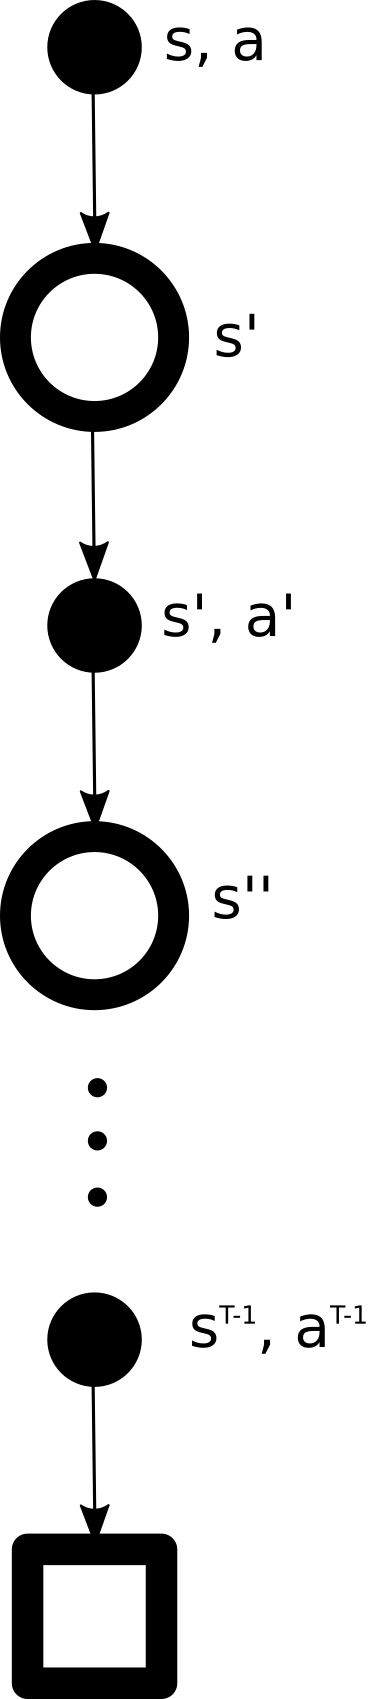
\includegraphics[scale=.4]{./backup_diagram.png}
\end{figure}
\subsection*{30. Exercise 5.9 Modify the algorithm for first-visit MC policy evaluation (Section 5.1) to use the incremental implementation for sample averages described in Section 2.4.}
\RestyleAlgo{boxruled}
\begin{algorithm}[ht]
\textbf{Input: a policy $\pi$ to be evaluated}\\
\textbf{Initialize:}\\
$V(s) \; \epsilon \; \mathbb{R}, \text{arbitrarily, for all } s\; \epsilon\; \mathcal{S}$\\
% $Returns(s) \leftarrow 0, \text{for all } s\; \epsilon \; \mathcal{S}$\\
$N(s) \leftarrow 0, \text{for all } s\; \epsilon \; \mathcal{S}$\\
	\For{ ever (for each episode)}
	{
		Generate an episode following $\pi:\; S_0, A_0,R_1, S_1, A_1,R_2,...,S_{T-1}, A_{T-1}, R_T $\\
		$G \leftarrow 0$ \\
		Loop for each step of episode, $t=T-1, T-2,...,0:$\\
		\quad $G\leftarrow \gamma G + R_{t+1}$\\
		\quad Unless $S_t$ appears in $S_0, S_1,...,S_{t-1}$:\\
		\quad \quad $N(S_t) \leftarrow N(S_t) + 1$ \\
%		\quad \quad $V(S_t) \leftarrow Returns(S_t) + \frac{1}{N(S_t)}[G - Returns(S_t)]$
		\quad \quad $V(S_t) \leftarrow V(S_t) + \frac{1}{N(S_t)}[G - V(S_t)]$
	}

 \caption{First-visit MC prediction with incremental update}
\end{algorithm}
\subsection*{31. Exercise 5.10 Derive the weighted-average update rule (5.8) from (5.7). Follow the pattern of the derivation of the unweighted rule (2.3). (Textbook p. 109)}
\begin{align*}
V_n &= \frac{\sum_{k=1}^{n-1}W_kG_k}{\sum_{k=1}^{n-1}W_k}, \quad \quad n \rightarrow n+1\\
V_{n+1} &= \frac{\sum_{k=1}^{n}W_kG_k}{\sum_{k=1}^{n}W_k} \\
&= \frac{1}{\sum_{k=1}^{n}W_k}\left[\sum_{k=1}^{n}W_kG_k\right]\\
&= \frac{1}{\sum_{k=1}^{n}W_k}\left[ W_nG_n + \sum_{k=1}^{n-1}W_kG_k \right]\\
&= \frac{1}{\sum_{k=1}^{n}W_k}\left[ W_nG_n + \frac{\sum_{k=1}^{n-1}W_k}{\sum_{k=1}^{n-1}W_k} \sum_{k=1}^{n-1}W_kG_k \right] \\
&= \frac{1}{\sum_{k=1}^{n}W_k}\left[ W_nG_n + V_n\sum_{k=1}^{n-1}W_k \right] \\
&= \frac{1}{\sum_{k=1}^{n}W_k}\left[ W_nG_n + V_n\sum_{k=1}^{n}W_k - V_nW_n \right]\\ 
&= V_n + \frac{W_nG_n}{\sum_{k = 1}^{n}W_k} - \frac{V_nW_n}{\sum_{k = 1}^{n}W_k} \\
&= V_n + \frac{W_n}{\sum_{k = 1}^{n}W_k}\left[ G_n - W_n \right] \\
&= V_n + \frac{W_n}{C_n}\left[ G_n - W_n \right],\quad \quad \text{with}\; C_n = \sum_{k=1}^n W_k \\
\end{align*}
\subsection*{33. Exercise 5.13 Show the steps to derive (5.14) from (5.12). (Textbook p. 114)}

\subsection*{34. Exercise 5.14 Modify the algorithm for off-policy Monte Carlo control (page 110) to use the idea of the truncated weighted-average estimator (5.10). Note that you will first need to convert this equation to action values.}
\newpage
\bibliographystyle{plainnat}
\bibliography{mybib}
\end{document}